% GenI-EG.tex
\begin{hcarentry}{GenI}
\label{geni}
\report{Eric Kow}%05/11
\makeheader

GenI is a surface realizer for Tree Adjoining Grammars.  Surface
realization can be seen a subtask of natural language generation
(producing natural language utterances, e.g., English texts, out of
abstract inputs).  GenI in particular takes a Feature Based
Lexicalized Tree Adjoining Grammar and an
input semantics (a conjunction of first order terms), and produces the
set of sentences associated with the input semantics by the grammar.  It
features a surface realization library, several optimizations, batch
generation mode, and a graphical debugger written in wxHaskell.  It was
developed within the TALARIS project and is free software licensed under
the GNU GPL, with dual-licensing available for commercial purposes.

Work on GenI has begun anew.  Since May 2011, Eric is working with
Computational Linguistics Ltd and SRI international to develop new
features for GenI and improve its scalability and performance for use in
an interactive tutoring application. We are excited to see GenI
potentially being used in the real world!

%**<img width=380 src="./GenI-main-screenshot.jpg">
%*ignore
\begin{center}
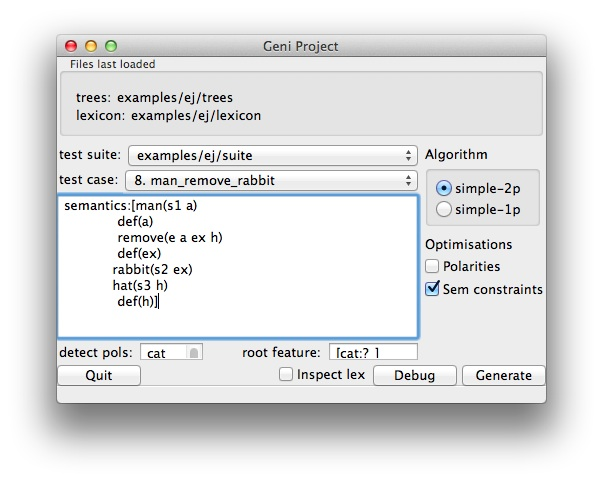
\includegraphics[width=0.4\textwidth]{html/GenI-main-screenshot.jpg}
\end{center}

%*endignore
%**<img width=380 src="./GenI-debugger-screenshot.jpg">
%*ignore
\begin{center}
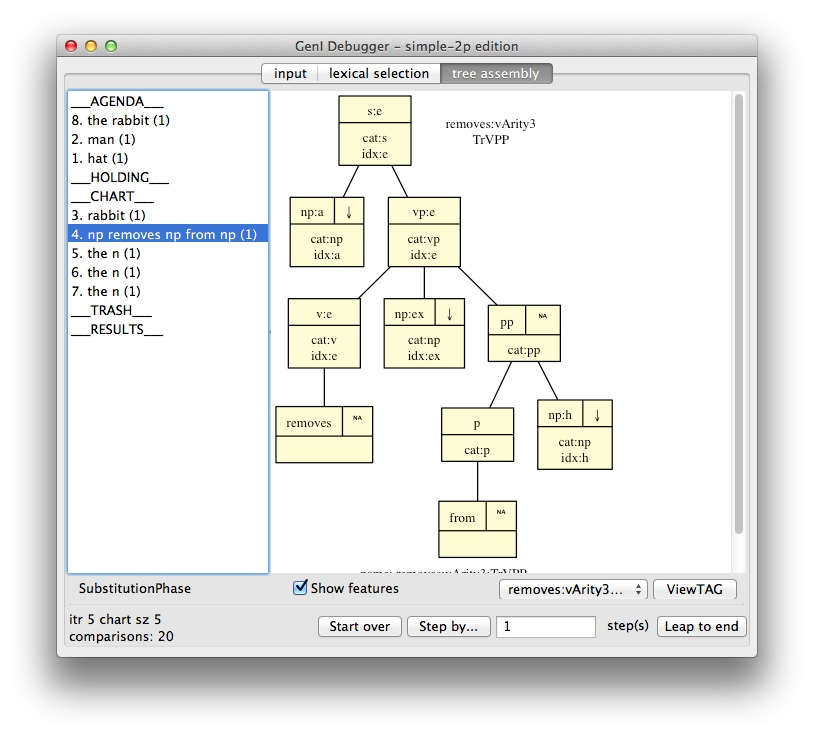
\includegraphics[width=0.4\textwidth]{html/GenI-debugger-screenshot.jpg}
\end{center}
%*endignore

GenI is available on Hackage, and can be installed via cabal-install.
Our most recent release of GenI was version 0.20.2 (2009-12-02), with
some bugfixes and simplifications.  For more information, please contact
us on the geni-users mailing list.

\FurtherReading
\begin{compactitem}
\item \url{http://projects.haskell.org/GenI}
\item Paper from Haskell Workshop 2006:

\url{http://hal.inria.fr/inria-00088787/en}
\item \url{http://websympa.loria.fr/wwsympa/info/geni-users}
\end{compactitem}
\end{hcarentry}
